\chapter{Design of Cloud-SAP}

\chapterintro{ This chapter introduces the high-level design of Cloud-SAP, highlighting its core concepts and indicating possible implementation ideas.
}

\section{Motivation}
Opis, ze wczesniejsze sa niewystarzcajace -> maja braki
Sys. autonomiczny lata te braki + mozna go zastosowac bo sa spelnione takie a takie wymagania (ich opis jest w blueprint)

\section{Overview}
Przedstawienie domeny - zasobow w naszym systemie, odniesienie tego do blueprint => wynikiem jest pomysl na system / diagram

ogolny opis systemu - jak sie odnosimy do CHOP, mamy 1 kontroler orkiestrujacy, kompletny system autonomiczny

\begin{figure}[!ht]
  \begin{center}
    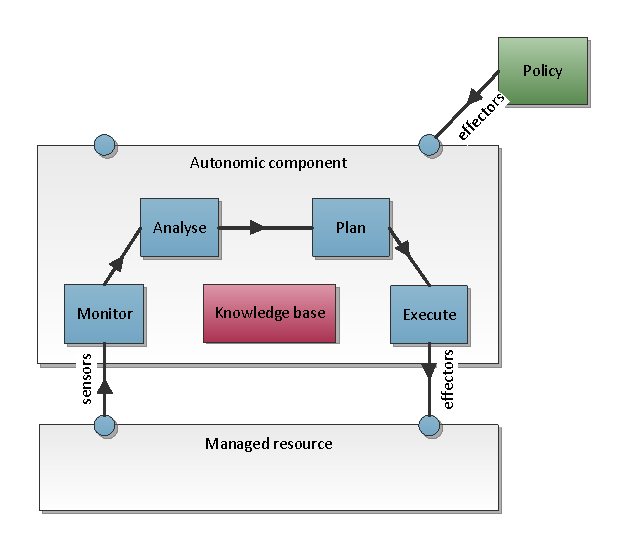
\includegraphics{chapter-design/autonomic-component}
  \end{center}
  \caption{autonomic component}
  \label{img:autonomic-component}
\end{figure}

% darek
\section{Application platform manager}
w kazdej sekcji opis MAPEK - co monitoruje, w jaki sposob analizuje i planuje, wykonuje

% darek
\section{Autonomic container manager}
It is expected that autonomic container manager supervises lifecycle of a container, modifying its properties accordingly to a current demand.

\subsection{Managed resource}
Container is an entity that provides an execution environment for an application platform. Whilst Cloud-SAP is a hypervisor agnostic, it is recommended to use operating system level virtualization technique instead of a full virtualization as a underlying mechanism for a container provisioning. Lightweight containers are more suitable for our needs especially because we rely entirely on Linux based operating system. Hence, it not necessary to use hardware-based hypervisor that supports other operating systems. Moreover, lightweight containers have been proved more effective in some scenarios: \cite{RaHiSj13}.

Container uses variety of underlying resources such as storage or network connection. However, for a simplicity, Cloud-SAP doesn't require autonomic container manager to manage them.

\subsubsection{Touchpoint}
Container's touchpoint externalises hypervisor and operating system APIs. Similarly to all touchpoints, two main parts can be distinguished:
\begin{itemize}
 \item \emph{sensors} - set of properties that expose system metrics such as CPU, memory, disk usage, network bandwidth
 \item \emph{effectors} - a collection of 'set' operations that aims to change container state: increase or decrease CPU or memory, for example. In fact, these operations directly corresponds to hypervisor capabilities.
\end{itemize}

It is highly recommended for sensors and effectors to be linked, forming together manageability capabilities. In other words, property (i.e. CPU) can be read only when it is possible to set it as well. 

\subsection{Autonomic controller}
Generally speaking, autonomic container controller aims to automate container's management function and externalise its configuration through its interfaces. In order to do achieve that, it implements a control loop that fully covers container life cycle: gathering information about it, analysing it, planning and executing actions on top of that. These four functions along with knowledge necessary to perform them designate modular structure of a controller as shown in figure \ref{img:autonomic-component}.

\subsubsection{Monitoring}
As it was already mentioned, monitoring module aims to gather data from container's sensors. While design of Cloud-SAP doesn't have any specific requirements regarding underlying monitoring mechanism, there are a few aspects that should be taken into consideration:
\begin{asparaenum}
  \item[\textbf{Data filters}]

  \item[\textbf{Persistence}]

  \item[\textbf{Standard compatibility}] Whilst there is no single, industry accepted standard of virtual machine monitoring, there were initiatives such as OCCI \cite{OCCI} that aims to close that gap. Having scaling across multiple cloud instances in mind, it is vital to provide compatibility at a container monitoring level. However, in some cases, standard-defined API may no be sufficient for a specific needs  
\end{asparaenum}


\subsubsection{Analysis}
\subsubsection{Planning}
\subsubsection{Execution}
\subsubsection{Knowledge}

% darek
\section{Autonomic stack manager}

% radek
\section{Autonomic cloud instance manager}

% radek
\section{Autonomic cloud federation manager}

\section{Summary}
podsumowanie, wyzwania stojace przed projektem, problemy ale takze obietnica dobrobytu i spokojnej starosci



